\documentclass[a4paper, 14pt, titlepage, fleqn]{extarticle}
\usepackage{style}
\usepackage{amsfonts}
\usepackage{float}
\usepackage{esint}
\usepackage{indentfirst}
\usepackage{setspace}
\usepackage{mathtools}
\usepackage{listings}
\DeclarePairedDelimiter\ceil{\lceil}{\rceil}
\DeclarePairedDelimiter\floor{\lfloor}{\rfloor}
\usepackage{color}


\definecolor{dkgreen}{rgb}{0,0.6,0}
\definecolor{gray}{rgb}{0.5,0.5,0.5}
\definecolor{mauve}{rgb}{0.58,0,0.82}

\lstset{frame=tb,
  language=C++,
  frame=single,
  aboveskip=3mm,
  belowskip=3mm,
  showstringspaces=false,
  columns=flexible,
  basicstyle={\small\ttfamily},
  numbers=none,
  keywordstyle=\color{blue},
  commentstyle=\color{dkgreen},
  stringstyle=\color{mauve},
  breaklines=true,
  breakatwhitespace=true,
  tabsize=1
}

\begin{document}
	\fefutitlepage{ОТЧЕТ}{к лабораторной работе №2\\по дисциплине <<Математическое моделирование>>}{01.03.02 <<Прикладная математика и информатика>>}{Б9120-01.03.02миопд}{Крюков Н.В.}
	\tableofcontents
	\newpage

    \onehalfspacing
    
    \sect{Введение}

        В данной лабораторной работе я буду решать задания, используя программы компьютерной математики. 
        Оформлять решенные задачи буду в среде компьютерной верстки <<\TeX>>, затем конвертировать в документ формата PDF.
        
    \sect{Задача о нагревательном приборе}

        \subsect{Постановка задачи}
            Необходимо получить график изменения температуры умного нагревательного прибора при условии всех теплопотерь. 
            Сам накревательный прибор может отключать свой нагревательный элемент при приближении к нужной температуре.
        
        \subsect{Выбор переменных}
            Множество нагревательных приборов и необходимых условий можно охарактеризовать параметрами
            
            \begin{enumerate}
                \item массой $m$;
                \item мощностью $p$;
                \item удельной теплоёмкостью материала $c$;
                \item коэффициентом конвективного теплообмена $k$;
                \item площадью поверхности нагревательного прибора $S$;
                \item температурой атмосферы $T_a$;
                \item температурой, до которой необходимо нагреть нагревательный прибор $T_R$.
            \end{enumerate}
            %Постоянная Стефана-Больцмана $\mathfrak{S} = 5.67 \cdot 10^{-8} \ \dfrac{\text{Вт}}{\text{м}^2 \cdot \text{K}^4}$.

        \subsect{Выбор законов и зависимостей}
            Для того, чтобы построить график изменения температуры, необходимо узнать, за счёт чего температура увеличивается и за счёт чего она может уменьшаться.
            При увеличении или уменьшении температуры количество тепла нагревательного прибора также увеличивается или уменьшается:
            \[\begin{split}
                & Q = c m T, \\
                & \left( Q_2 - Q_1 \right) = c m \left( T_2 - T_1 \right), \\
                & \Delta Q = c m \Delta T. \\
            \end{split}\]
            Уменьшение температуры может происходить по нескольким причинам: конвекция и тепловое излучение. 
            Формула конвективного теплообмена за единицу времени -- \( k S \left( T - T_a \right) \Delta t \).
            Формула теплового излучения за единицу времени -- \( S \mathfrak{S} \left( T^4 - T_a^4 \right) \Delta t \).
            Переобозачим суммарные теплопотери за единицу времени как $L\left( T \right) \cdot \Delta t$.
            
            Увеличение количества тепла происходит за счёт мощности на единицу времени \(P \cdot \Delta t\).
            Предположим, что нагревательный элемент может отключаться, тогда домножим предыдущую формулу на некий коэффициент $H$, который будет меняться с изменениями температуры -- \( P \cdot \Delta t \cdot H \).
            
        \subsect{Формулировка математической модели}
            % Чтобы нагревательный прибор мог поддерживать 
        
            Узнаем сколько тепла получает и отдаёт нагревательный прибор
            \[ Q = P \cdot \Delta t - L\left( T \right) \cdot \Delta t \]

            Подставим формулу количества тепла нагревательного элемента:
            \[c m \Delta T = P \cdot \Delta t - L\left( T \right) \cdot \Delta t \]

            Преобразуем уравнение:
            \[ \dfrac{\Delta T}{\Delta t} = \dfrac{P - L\left( T \right)}{c m} \]

            Предположим существование функции \(H\), которая изменяет работу нагревательного элемента.
            \[ \dfrac{\Delta T}{\Delta t} = \dfrac{P \cdot H - L\left( T \right)}{c m} \]

            Пусть при преодолении необходимой температуры функция $H$ равна нулю, в остальных случаях -- единице.
            Если $t > T_R$ тогда 0, иначе 1:
            \[ H = 1 - \floor*{\dfrac{t}{T_R}} \]

            Финальная формула выглядит так:

            \[ \dfrac{\Delta T}{\Delta t} = \dfrac{P \cdot \left(1 - \floor*{\tfrac{t}{T_R}}\right) - k S \left( T - T_a \right) - S \mathfrak{S} \left( T^4 - T_a^4 \right)}{c m} \]

            Математическая модель поставлена

        \subsect{Решение}

            Последнее уравнение является дифференциальным уравнением температуры по времени.
            Так как в начальный момент времени $t_0$ температура равна атмосферной $T = T_a$, то значит эта задача является задачей Коши.
            Напишем программу для высчитывания графика роста температуры. 
            
            % \begin{enumerate}
            %     \item массой $m = 1 \ \text{килограмм}$;
            %     \item количеством нагревательных элементов в нагревательном приборе $n = 10 \ \text{шт}$
            %     \item мощностью $p = 3000 \ \text{Вт}$;
            %     \item материалом прибора - железо;
            %     \item удельной теплоёмкостью материала $c = 460 \ \dfrac{\text{Дж}}{\text{кг} \cdot \text{с}}$;
            %     \item коэффициентом конвективного теплообмена $k = 25 \ \dfrac{\text{Вт}}{\text{м}^2 \cdot \text{K}}$;
            %     \item площадью поверхности нагревательного прибора $S = 0.01 \ \text{м}^2$;
            %     \item температурой атмосферы $T_a = 300 \ \text{K}$;
            %     \item температурой, до которой необходимо нагреть нагревательный прибор $T_R = 600 \ \text{K}$.
            % \end{enumerate}

        \subsect{Код программы}

    \begin{lstlisting}
    #include <iostream>
    #include <fstream>
    #include <cmath>
    #include <string>
    
    int m = 1;
    int p = 3000;
    int c = 460;
    int tA = 300;
    double k = 25;
    double s = 0.05;
    const double sigma = 5.7 * pow(10, -8);
    int tR = 600;
    
    using std::cin;
    using std::cout;
    using std::endl;
    using std::string;
    using std::ofstream;
    using std::to_string;
    
    double losses(double t) {
        return s * (k * (t - tA) + sigma * (pow(t, 4) - pow(tA, 4)));
    }
    
    double h(double t) {
        return t >= tR ? 0 : 1;
    }
    
    double f(double t) {
        return (1.0 * (1.0 * p * h(t) - losses(t)) / (c * m));
    }
    
    int main() {
        ofstream fout("output.txt");
        string x = "";
        string y = "";
        double t = tA;
        for (int i = 0; i < 100; i++) {
            cout << i << ' ' << h(t) << ' ' << t << ' ' << f(t) << endl;
            x += to_string(i);
            x += ", ";
            y += to_string(t);
            y += ", ";
            t += (double)f(t);
        }
        fout << x << endl << y << endl;
        fout.close();
    }

    \end{lstlisting}

        \subsect{Тестирование}
            Проведём эксперимент с конкретными значениями

            Для визуализации результатов использовалась библиотека языка Python

            \begin{figure}[H]
                \centering
                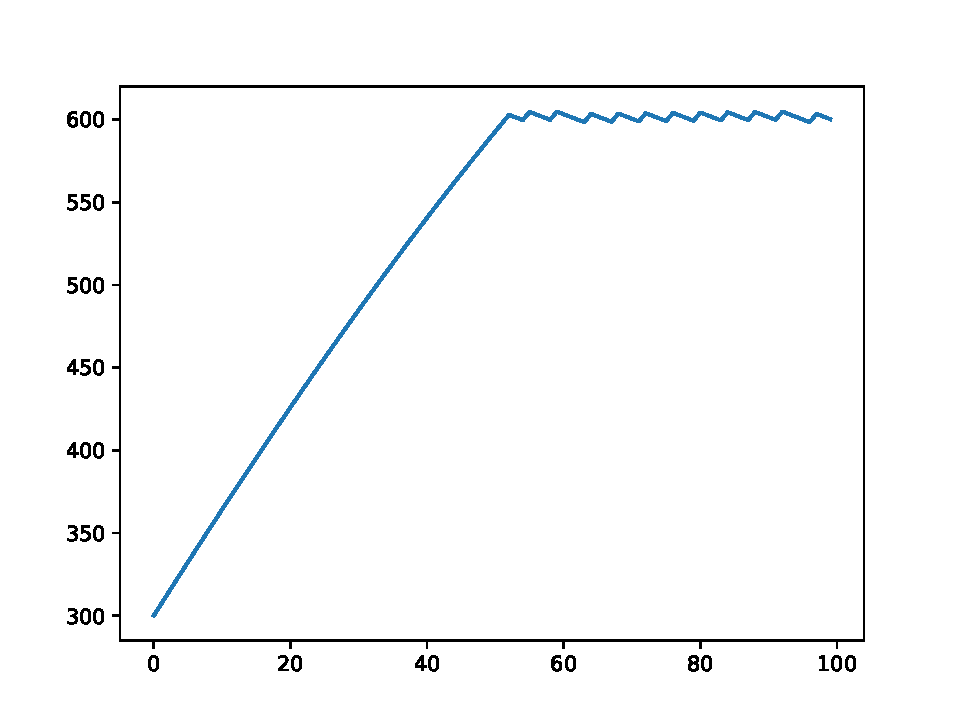
\includegraphics[width = \textwidth]{assets/nag1t100.pdf}
                \caption[.] {График температуры}
            \end{figure}          

    \sect{Заключение}
        
        В ходе работы была написана и протестирована программа для прогнозирования температуры нагревательного прибора. 

\end{document}